% coding:utf-8
\section{Taylorreihen}
Ein Ausdruck der Form 
\[ \boxed{f(x) = \sum_{n = 0}^{\infty} a_n x^n = a_0 + a_1 x + a_2 x^2 + a_3 x^3 \dots a_n x^n} \]
\[ \boxed{a_k = \frac{f^{(K)}(x_0)}{K!}} \]
nennt man eine Potenzreihe

\subsection{Konvergenzradius}
Der Konvergenzradius sagt aus, innerhalb von welchem Intervall (ausgehend vom Approximationspunkt)
eine Potenzreihe konvergiert. Der Begriff Radius ist dabei ein Skalar auf $\Omega$ und nicht im $\mathbb{R}^2$.

\begin{figure}[h!]
\centering
% 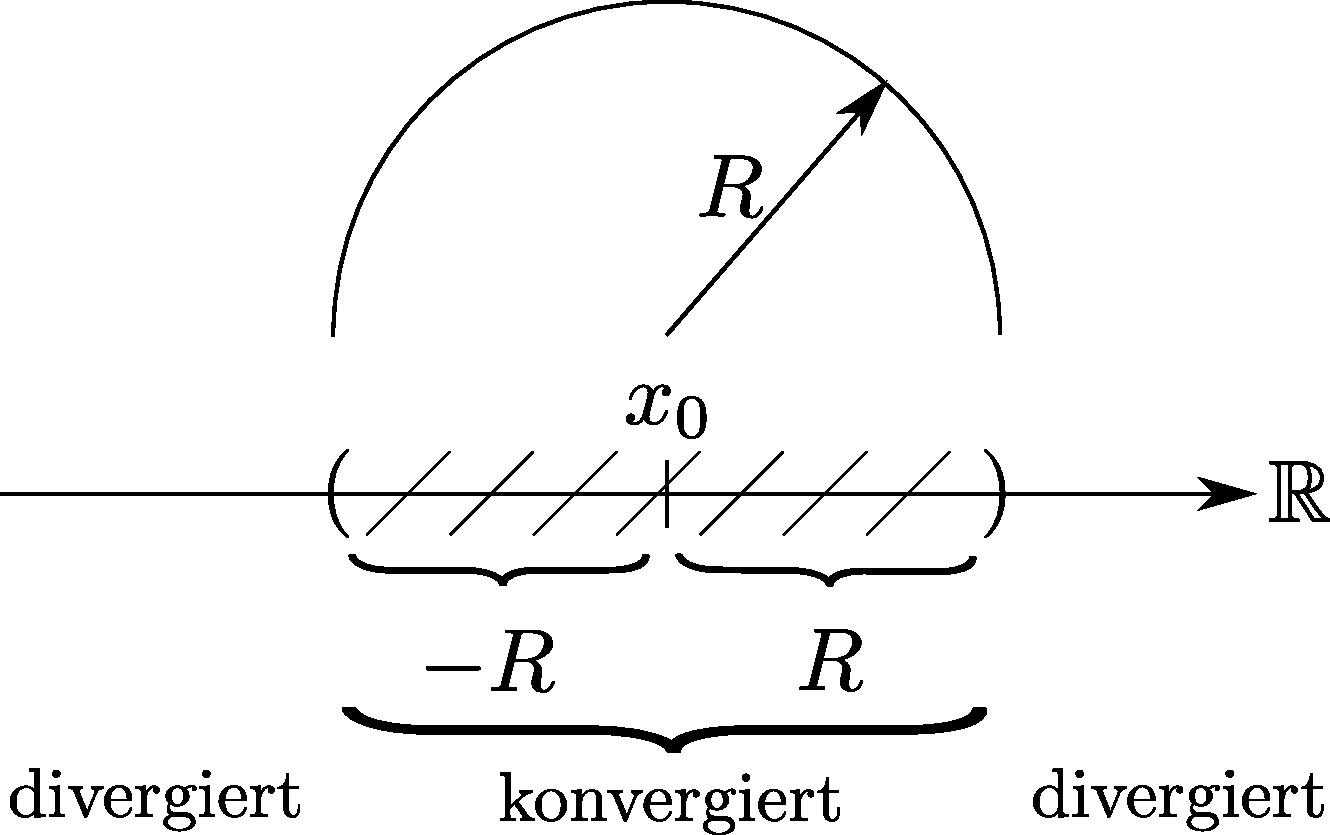
\includegraphics[width=0.6\textwidth]{konvergenzradius.pdf}
\end{figure}

\[ \boxed{ \begin{array}{lll} 
    |x| < R & \Rightarrow & \text{Potenzreihe ist konvergent} \\
    |x| > R & \Rightarrow & \text{Potenzreihe ist divergent} \\
    |x| = R & \Rightarrow & \text{überprüfen was für $x=R$ und $-x=R$ gilt}
\end{array} } \]

\[ \boxed{a_k = \frac{f^{(K)}(x_0)}{K!}} \]
\[ \boxed{R = \frac{1}{q} = \lim_{n \rightarrow \infty} \left| \frac{a_n}{a_{n + 1}} \right|} \]

\subsection{Taylorreihe mit Entwicklungspunkt $x_0 = 0$}
Eine Taylorreihe mit Entwicklungspunkt $x_0 = 0$ wird auch MacLaurin-Reihe genannt
\[ \boxed{f(x) = \sum_{K=0}^{\infty}\frac{f^{(K)}(0)}{K!} x^K} \]

\subsection{Taylorreihe mit Entwicklungspunkt $x_0 \neq 0$}
\[ \boxed{f(x) = \sum_{K=0}^{\infty}\frac{f^{(K)}(x_0)}{K!}\cdot (x-x_0)^K} \]

\subsection{Einfache Funktionen als Taylorreihen}
\[ \boxed{e^x = \sum_{K=0}^{\infty} \frac{x^K}{K!}} \]
\[ \boxed{\sin(x) = \sum_{K=0}^{\infty} \frac{(-1)^K x^{2K+1}}{(2K+1)!}} \]
\[ \boxed{\cos(x) = \sum_{K=0}^{\infty} \frac{(-1)^K x^{2K}}{(2K)!}} \]
\[ \boxed{\cosh(x) = \sum_{K=0}^{\infty} \frac{x^{2K}}{(2K)!}} \]
\[ \boxed{\sinh(x) = \sum_{K=0}^{\infty} \frac{x^{2K+1}}{(2K+1)!}} \]

\subsection{Kochrezept Taylorreihen}
\begin{enumerate}
  \item Stelle finden, an welcher die Funktion approximiert werden soll. 
  \item Bereich und Genauigkeit bzw. Fehler definieren oder den Grad der Potenzreihe fix wählen. 
\end{enumerate}

\ifti
\subsection{Taylorreihe mit dem TI-89 berechnen}
\begin{verbatim}
taylor(Funktion,Variable,Ordnung[,Punkt])
\end{verbatim}
Funktion: Funktion, zu welcher die Taylorreihe gesucht ist. \\
Variable: Variable in Funktion\\
Ordnung: Ordnung der Taylorreihe\\
Punkt: Optional: Punkt, an dem Die Funktion approximiert wird. (Default: 0)
\fi
\ifnspire
\subsection{Taylorreihe mit dem TI-Nspire berechnen}
\begin{verbatim}
taylor(Funktion,Variable,Ordnung[,Punkt])
\end{verbatim}
Funktion: Funktion, zu welcher die Taylorreihe gesucht ist. \\
Variable: Variable in Funktion\\
Ordnung: Ordnung der Taylorreihe\\
Punkt: Optional: Punkt, an dem Die Funktion approximiert wird. (Default: 0)
\fi
